\documentclass{article}
\usepackage[utf8]{inputenc}
\usepackage{graphicx}
\usepackage{amssymb}

\title{\textbf{Rod Cutting Problem By Using Dynamic Programming}}
\author{Saeah Go}
\date{November 12th 2021}

\begin{document}

\maketitle

\section{\textbf{Abstract}}
\indent \indent The problem of cutting a rod into rods of smaller length in way that maximizes their total value. We develop a rod cutting problem using dynamic programming and bottom up method. Dynamic programming is an algorithm design technique, is a technique for solving problems with overlapping sub-problems. \\ \indent Dynamic programming suggest solving each of the smaller sub-problems only once and recording the results in a table from which a solution to the original problem can then be obtained. So we can say that it is a general method for optimizing multistage decision processes. Rod cutting problem is an example uses dynamic programming to solve a simple problem in deciding where to cut steel rods. \\

\section{\textbf{Introduction}}
\indent \indent Basic idea of Rod-Cutting Problem is that a company buys long steel rods and cuts them into shorter rods, which it then sells. We assume that each cut is free. The company wants to know the best way to cut up the rods for a maximum profit. \\
\indent We assume that we know, for $i = 1, 2, \ldots ,$ the price $p_i$ in dollars that the company charges for a rod of length $i$ inches. Also assume that the rod lengths are always a natural number. So the rod-cutting problem is given a rod of length $n$ inches and a table of prices $p_i$ for $i = 1, 2, \ldots, n$, determine the maximum revenue $r_n$ obtainable by cutting up the rod and selling the pieces. We should note that if the price $p_n$ for a rod of length $n$ is large enough, an optimal solution may require no cutting at all. \\
\indent In the report, the rod cutting problem by bottom up method is presented and analyzed. We will test $9$ cases and record the running time for those cases. We will figure out whether the best and worst cases must be the same in this problem. So our hypothesis is the best and worst cases should be the same. We will show whether our experimental results support our hypothesis. (confirmed or dis-confirmed) 

\section{\textbf{Background}}
\indent \indent Since we are using dynamic programming for optimal rod cutting, computed solutions to sub-problems are stored in a table so that these don't have to be recomputed. (In other words, each sub-problem to be solved only once, and saving its solution). So note that dynamic programming is not useful when there are no common (overlapping) because there is no point storing the solutions if they are not needed again. \\
\indent Anyway dynamic programming thus uses additional memory to save computation time. In other words, the bottom up method requires $O(n)$ extra space, where $n$ is the rod length. \\
\indent There are two approaches for rod cutting problem, one is top down (memoization) and the other is bottom up (tabulation). In this report we implemented using the bottom up method. The running time of procedure bottom up cut rod is $O(n^2)$, since it has two nested for loops.


\section{\textbf{Data Analysis Process or Procedure}}
\indent \indent We did this experiment with a few cases of small inputs. Since our inputs are size $n$ and price array $p$, we didn't need to consider other types of input. (For example, character type, etc.) We decided to test a bunch of cases and from four to sixteen. In each case, we checked the running time to show the time complexity and also checked whether we get the maximum obtainable values. \\
\indent So for the performance testing, we checked whether we get the correct maximum obtainable values or not. Not only performance testing, but we also had to measure the time. Timing data is collected by measuring the starting time using time.time() function in the time package. So we loaded the time package using "import time". After the cutting process, we used the time.time() function again to check the execution time and subtract those to get the running time. 
Now let's look at the procedures by checking the test cases one by one.

\subsection{\textbf{Size 4}}
\begin{center}
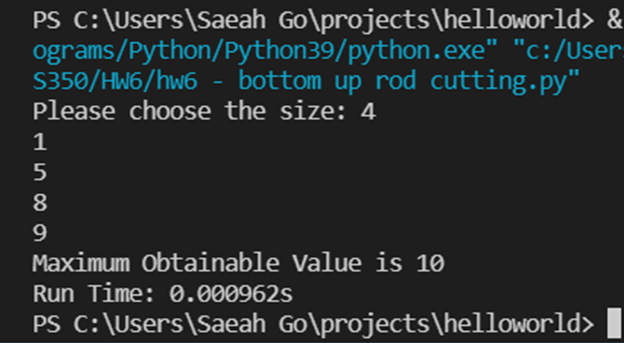
\includegraphics[scale = 0.7]{size 4.png} \\
\end{center}
The price array is $p = [1, 5, 8, 9]$. The maximum obtainable value is 10, because we can cut them half then 5 + 5 = 10. It takes 0.000962 seconds. 

\subsection{\textbf{Size 5}}
\begin{center}
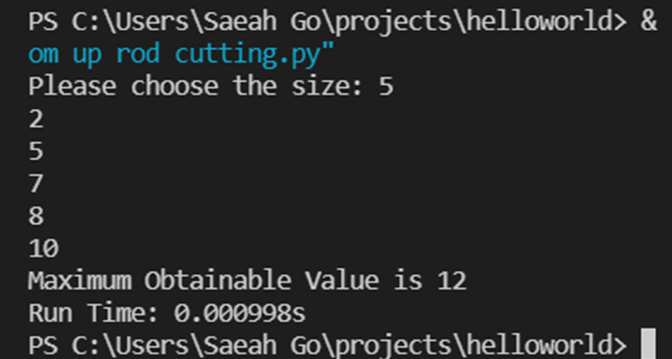
\includegraphics[scale = 0.7]{size 5.png} \\
\end{center}
The price array is $p = [2, 5, 7, 8, 10]$. As we can see, the maximum obtainable value is 12, if we cut 5 inches long rod into two pieces (one is 2 inches and the other is 3 inches), then the price is 5 + 7 = 12 so \$12 dollars. We can check that the execution time is 0.000997 seconds.

\subsection{\textbf{Size 6}}
\begin{center}
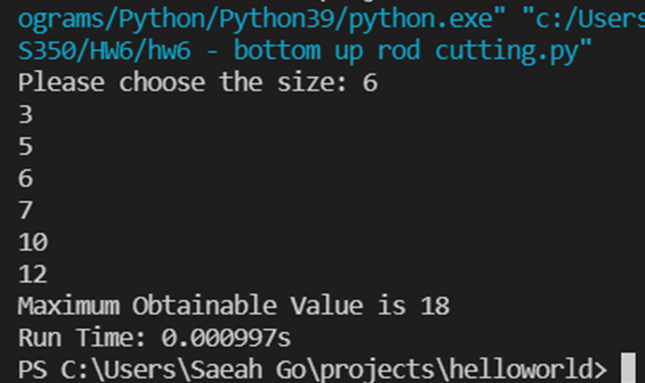
\includegraphics[scale = 0.7]{size 6.png} \\
\end{center}
The price array is $p = [3, 5, 6, 7, 10, 12]$. The maximum obtainable value is $\$18$ dollars, since if I cut it into six pieces, $3 \times 6 = 18$. We can see that it takes $0.000997$ seconds.

\subsection{\textbf{Size 7}} 
\begin{center}
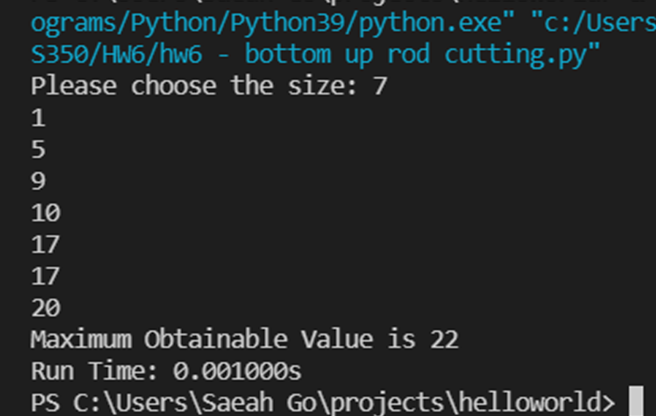
\includegraphics[scale = 0.7]{size 7.png} \\
\end{center}
The input array (price array) is $p = [1, 5, 9, 10, 17, 17, 20]$. The maximum obtainable value is $22$ dollars, since if we cut the rod into two parts, with 2 inches one and 5 inches one, we get $\$5 + \$17 = \$22.$ The execution time for input size $7$ is $0.001$ seconds.

\subsection{\textbf{Size 8}}
\begin{center}
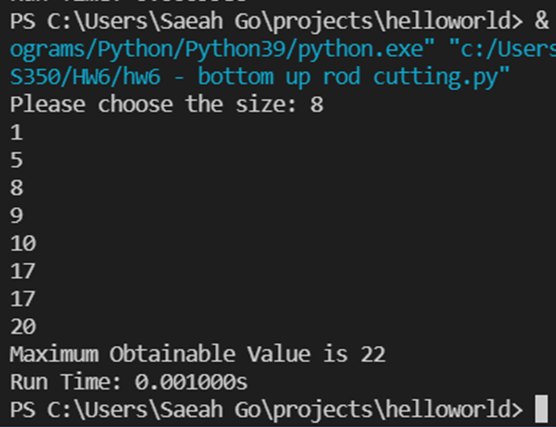
\includegraphics[scale = 0.6]{size 8.png} \\
\end{center}
In this case, the price array is $p = [1, 5, 8, 9, 10, 17, 17, 20]$. The maximum obtainable value is $22$ dollars. Because if we cut the rod into two pieces, one with $2$ inches and the other is $6$ inches, then the price would be $5 + 17 = 22$. We can check the execution time is $0.001$ seconds.

\subsection{\textbf{Size 10}}
\begin{center}
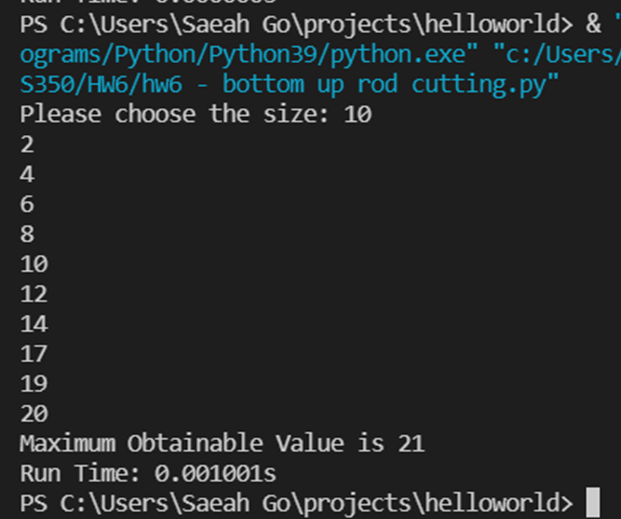
\includegraphics[scale = 0.5]{size 10.png} \\
\end{center}
The input array for this input size 10 is $p = [2, 4, 6, 8, 10, 12, 14, 17, 19, 20]$. The maximum obtainable value is 21, since if we cut it to two pieces (1 inch and 9 inches) we get 2 + 19 = 21 dollars. This time the running time is 0.001 seconds again.

\subsection{\textbf{Size 12}} 
\begin{center}
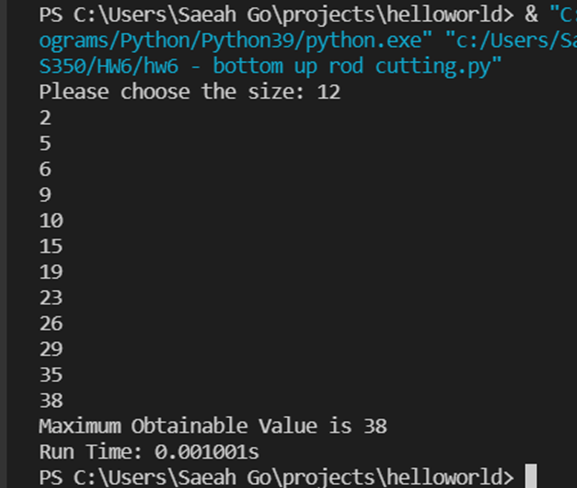
\includegraphics[scale = 0.5]{size 12.png} \\
\end{center}
The input price array is $p = [2, 5, 6, 9, 10, 15, 19, 23, 26, 29, 35, 38]$. The maximum obtainable value is 38, because when we didn't cut it, it's the maximum profit. The running time is 0.001001 seconds. 

\subsection{\textbf{Size 14}}
\begin{center}
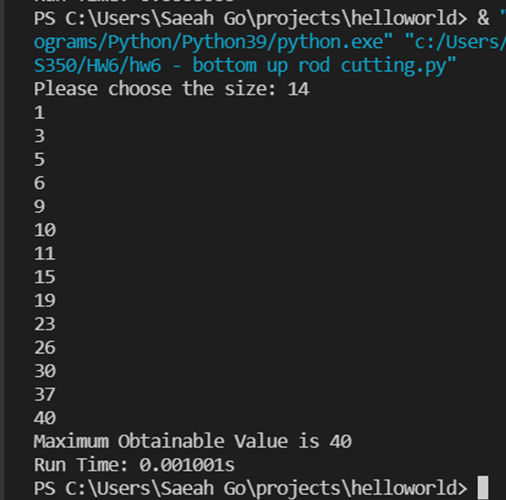
\includegraphics[scale = 0.5]{size 14.png} \\
\end{center}
Input array p is $p = [1, 3, 5, 6, 9, 10, 11, 15, 19, 23, 26, 30, 37, 40]$. The maximum obtained value for size 14 is 40, we get a maximum profit when we do not cut the rod. And again, the execution time is 0.001001 seconds. 

\subsection{\textbf{Size 16}}
\begin{center}
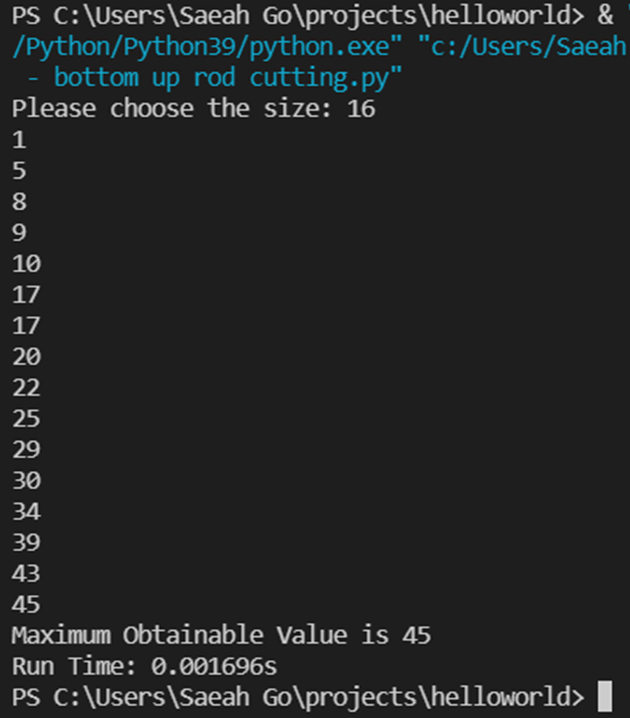
\includegraphics[scale = 0.4]{size 16.png} \\
\end{center}
Price array $p$ is $p = [1, 5, 8, 9, 10, 17, 17, 20, 22, 25, 29, 30, 34, 39, 43, 45]$. The maximum obtainable value is again, 45. Since we get the maximum profit 45 when we don't cut the rod. The execution time in this case is 0.001696 seconds.

\section{\textbf{Analysis Results}}
\indent Based on the test performance results, we made a graph in R and we got: \\
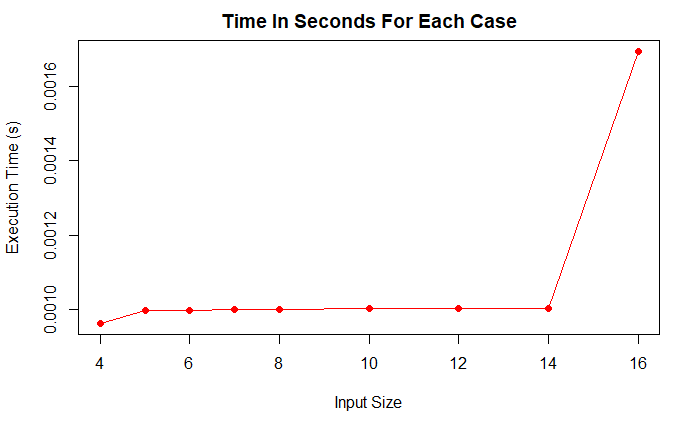
\includegraphics[scale = 0.65]{graph.png} \\
\indent To explain what the case number denotes briefly, the $x$-axis indicates the input sizes. Since we considered input cases from $4$ to $16$, we can check it. The $y$-axis is the execution time in seconds. In the graph, we can see that the running time is getting bigger as the input size grows. Even though we got a really big execution time value for the input $16$, at least we can see the $n^2$ growth for this. In dynamic programming problems, time complexity is the number of unique states/sub-problems $\times$ time taken per state. So we should consider all the cases as random cases (average cases). In other words, the best and worst cases are the same. And since we used two for loops, for loop in for loop, the time complexity for this problem is $O(n^2)$. Overall the performance testing went well and we got reasonable values of the running time. We saw the results what we expected before the experiment.

\section{\textbf{Recommendations}}
\indent \indent As I briefly mentioned in the Introduction part, dynamic programming is not useful when there are no common (overlapping) because there is no point storing the solutions if they are not needed again. But in this case, as we store the value in the array $val[]$, and we can use it again and again, it is really useful. Even though rod cutting is a kind of problem which can be solved without using dynamic programming, I really recommend to use dynamic programming since we can optimize it greatly by using it.  

\section{\textbf{Appendix}} 
\begin{center}
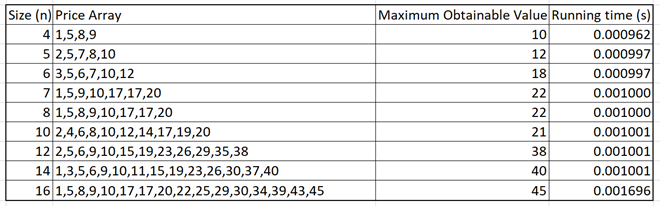
\includegraphics[scale = 0.7]{table} \\
\scriptsize{Table 1}
\end{center}
\indent \indent This is the table of raw data, the first column shows the input size n (the length of rod). The second column, Price Array, shows the prices for each inch. The third column Maximum Obtainable Value shows the maximum profits we could get. The last column, Running time shows the execution time for each case.
\end{document}


